\documentclass{beamer}
\setbeamersize{text margin left=5mm,text margin right=5mm}
\usepackage[utf8]{inputenc}
\usepackage{xcolor}
\usepackage{ulem} % strikeout

\usepackage{tikz}
\usetikzlibrary{arrows,shapes,tikzmark}
\usepackage{attachfile}

\renewcommand{\today}{\number \day \ \ifcase \month \or January\or February\or March\or %
April\or May \or June\or July\or August\or September\or October\or November\or %
December\fi \ \number \year}

%Information to be included in the title page:
\title{Data Types}
\author{Richard Zak}
\institute{UMBC}
\date{\today}
\begin{document}

%\frame{\titlepage}

\begin{frame}
Consider these numbers in memory. What do they mean?
\begin{table}[]
\begin{tabular}{|l|l|l|l|l|l|l|l|l|}
\hline
 \texttt{0x00} & \texttt{0x01} & \texttt{0x02} & \texttt{0x03} & \texttt{0x04} & \texttt{0x05} & \texttt{0x06} & \texttt{0x07} &
 \texttt{0x08} \\
\hline 
\end{tabular}
\end{table}
\end{frame}

\begin{frame}{Char - 8 bits, 1 byte}

\begin{table}[]
\begin{tabular}{|l|l|l|l|l|l|l|l|l|}
\hline
 \color{red}\texttt{0x00} & \texttt{0x01} & \texttt{0x02} & \texttt{0x03} & \texttt{0x04} & \texttt{0x05} & \texttt{0x06} & \texttt{0x07} &
 \texttt{0x08} \\
\hline 
\end{tabular}
\end{table}

\begin{table}[]
\begin{tabular}{c r r}
Format & Little Endian & Big Endian \\
\hline
Value &  0   & 0 \\
Order & 0x00 & 0x00
\end{tabular}
\end{table}

\end{frame}

\begin{frame}{Array of Chars}

\begin{table}[]
\begin{tabular}{|l|l|l|l|l|l|l|l|l|}
\hline
 \tikz[baseline, remember picture] \node[anchor=base] (t1) {\color{red}\texttt{0x00}}; & \color{blue}\texttt{0x01} & \color{green}\texttt{0x02} & \color{red}\texttt{0x03} & \color{blue}\texttt{0x04} & \color{green}\texttt{0x05} & \color{red}\texttt{0x06} & \color{blue}\texttt{0x07} &
 \color{green}\texttt{0x08} \\
\hline 
\end{tabular}
\end{table}

\begin{table}[]
\begin{tabular}{c r r}
Index & Little Endian & Big Endian \\
\hline
0\tikz[remember picture] \node[coordinate,anchor=west] (n1) {}; & 0 & 0 \\
1 & 1 & 1 \\
2 & 2 & 2 \\
3 & 3 & 3 \\
4 & 4 & 4 \\
5 & 5 & 5 \\
6 & 6 & 6 \\
7 & 7 & 7 \\
8 & 8 & 8 \\
\end{tabular}
\end{table}

\begin{tikzpicture}[remember picture,overlay]   %% use here too
        \path[draw=red,thin,->] -- ([xshift=-1mm] n1.west) to (t1.south);
\end{tikzpicture}

\end{frame}

\begin{frame}{Short Integer - 16 bits, 2 bytes}

\begin{table}[]
\begin{tabular}{|l|l|l|l|l|l|l|l|l|}
\hline
 \color{red}\texttt{0x00} & \color{red}\texttt{0x01} & \texttt{0x02} & \texttt{0x03} & \texttt{0x04} & \texttt{0x05} & \texttt{0x06} & \texttt{0x07} &
 \texttt{0x08} \\
\hline 
\end{tabular}
\end{table}

\begin{table}[]
\begin{tabular}{c r r}
Format & Little Endian & Big Endian \\
\hline
Value &  256   & 1 \\
Order & 0x0100 & 0x0001
\end{tabular}
\end{table}

\end{frame}

\begin{frame}{Array of Short Integers}

\begin{table}[]
\begin{tabular}{|l|l|l|l|l|l|l|l|l|}
\hline
 \color{red}\texttt{0x00} & \color{red}\texttt{0x01} & \tikz[baseline, remember picture] \node[anchor=base] (t1){\color{blue}\texttt{0x02}}; & \color{blue}\texttt{0x03} & \color{green}\texttt{0x04} & \color{green}\texttt{0x05} & \color{red}\texttt{0x06} & \color{red}\texttt{0x07} &
 \sout{\texttt{0x08}} \\
\hline 
\end{tabular}
\end{table}

\begin{table}[]
\begin{tabular}{c r r}
Index & Little Endian & Big Endian \\
\hline
 0 & 256 & 1 \\
 1\tikz[remember picture] \node[coordinate,anchor=west] (n1) {}; & 770 & 515 \\
 2 & 1284 & 1029 \\
 3 & 1798 & 1543
\end{tabular}
\end{table}

\begin{tikzpicture}[remember picture,overlay]   %% use here too
        \path[draw=red,thin,->] -- ([xshift=-2mm,yshift=1mm] n1.west) -- ([xshift=-30pt,yshift=30pt]n1.west) node[above left]{}  -- (t1.south);
\end{tikzpicture}

\end{frame}

\begin{frame}{Integer - 32 bits, 4 bytes}

\begin{table}[]
\begin{tabular}{|l|l|l|l|l|l|l|l|l|}
\hline
 \color{red}\texttt{0x00} & \color{red}\texttt{0x01} & \color{red}\texttt{0x02} & \color{red}\texttt{0x03} & \texttt{0x04} & \texttt{0x05} & \texttt{0x06} & \texttt{0x07} &
 \texttt{0x08} \\
\hline 
\end{tabular}
\end{table}

\begin{table}[]
\begin{tabular}{c r r}
Format & Little Endian & Big Endian \\
\hline
Value &  50,462,976   & 66,051 \\
Order & 0x03020100 & 0x00010203
\end{tabular}
\end{table}

\end{frame}

\begin{frame}{Array of Integers}

\begin{table}[]
\begin{tabular}{|l|l|l|l|l|l|l|l|l|}
\hline
 \color{red}\texttt{0x00} & \color{red}\texttt{0x01} & \color{red}\texttt{0x02} & \color{red}\texttt{0x03} & \color{blue}\texttt{0x04} & \color{blue}\texttt{0x05} & \color{blue}\texttt{0x06} & \color{blue}\texttt{0x07} &
 \sout{\texttt{0x08}} \\
\hline 
\end{tabular}
\end{table}

\begin{table}[]
\begin{tabular}{c r r}
Index & Little Endian & Big Endian \\
\hline
  0 & 50,462,976 & 66,051 \\
  1 & 117,835,012  & 67,438,087
\end{tabular}
\end{table}

\end{frame}

\begin{frame}{Long Integer - 64 bits, 8 bytes}

\begin{table}[]
\begin{tabular}{|l|l|l|l|l|l|l|l|l|}
\hline
 \color{red}\texttt{0x00} & \color{red}\texttt{0x01} & \color{red}\texttt{0x02} & \color{red}\texttt{0x03} & \color{red}\texttt{0x04} & \color{red}\texttt{0x05} & \color{red}\texttt{0x06} & \color{red}\texttt{0x07} &
 \sout{\texttt{0x08}} \\
\hline 
\end{tabular}
\end{table}

\begin{table}[]
\begin{tabular}{c r r}
Format & Little Endian & Big Endian \\
\hline
Value &  506,097,522,914,230,528   & 283,686,952,306,183 \\
Order & 0x0706050403020100 & 0x0001020304050607
\end{tabular}
\end{table}

\end{frame}

\begin{frame}{Floating Point Value - 32 bits, 4 bytes}

\begin{table}[]
\begin{tabular}{|l|l|l|l|l|l|l|l|l|}
\hline
 \color{red}\texttt{0x00} & \color{red}\texttt{0x01} & \color{red}\texttt{0x02} & \color{red}\texttt{0x03} & \texttt{0x04} & \texttt{0x05} & \texttt{0x06} & \texttt{0x07} &
 \texttt{0x08} \\
\hline 
\end{tabular}
\end{table}

\begin{table}[]
\begin{tabular}{c r r}
Format & Little Endian & Big Endian \\
\hline
Value &  3.820471434542632e-37   & 9.25571648671185e-41 \\
Order & 0x03020100 & 0x00010203
\end{tabular}
\end{table}

\end{frame}

\begin{frame}{Array of Floating Point Values - 32 bits, 4 bytes}

\begin{table}[]
\begin{tabular}{|l|l|l|l|l|l|l|l|l|}
\hline
 \color{red}\texttt{0x00} & \color{red}\texttt{0x01} & \color{red}\texttt{0x02} & \color{red}\texttt{0x03} & \color{blue}\texttt{0x04} & \color{blue}\texttt{0x05} & \color{blue}\texttt{0x06} & \color{blue}\texttt{0x07} &
 \sout{\texttt{0x08}} \\
\hline 
\end{tabular}
\end{table}

\begin{table}[]
\begin{tabular}{c r r}
Index & Little Endian & Big Endian \\
\hline
0 &  3.820471434542632e-37   & 9.25571648671185e-41 \\
1 & 1.0082513512365273e-34 & 1.5636842486455404e-36
\end{tabular}
\end{table}

\end{frame}

\begin{frame}{Double-Precision Floating Point Value - 64 bits, 8 bytes}

\begin{table}[]
\begin{tabular}{|l|l|l|l|l|l|l|l|l|}
\hline
 \color{red}\texttt{0x00} & \color{red}\texttt{0x01} & \color{red}\texttt{0x02} & \color{red}\texttt{0x03} & \color{red}\texttt{0x04} & \color{red}\texttt{0x05} & \color{red}\texttt{0x06} & \color{red}\texttt{0x07} &
 \sout{\texttt{0x08}} \\
\hline 
\end{tabular}
\end{table}

\begin{table}[]
\begin{tabular}{c r r}
Format & Little Endian & Big Endian \\
\hline
Value &  7.949928895127363e-275   & 1.40159977307889e-309 \\
Order & 0x0706050403020100 & 0x0001020304050607
\end{tabular}
\end{table}

\end{frame}

\begin{frame}{Data Types}
\begin{table}[]
\begin{tabular}{c c r r}
Type & Bytes & Min & Max \\
\hline
char & 1 & -127 & +127 \\
unsigned char & 1 & 0 & +255 \\
short & 2 & -32,767 & +32,767   \\
unsigned short & 2 & 0 & +65,535 \\
int & 4 & -2,147,483,647 & +2,147,483,647 \\
unsigned int & 4 & 0 & +4,294,967,295
\end{tabular}
\end{table}
long: 8 bytes, 64-bit \\
long min: -9,223,372,036,854,775,808 \\
long max: +9,223,372,036,854,775,807 \\
unsigned long max: +18,446,744,073,709,551,615
\end{frame}

\begin{frame}{Data Types}
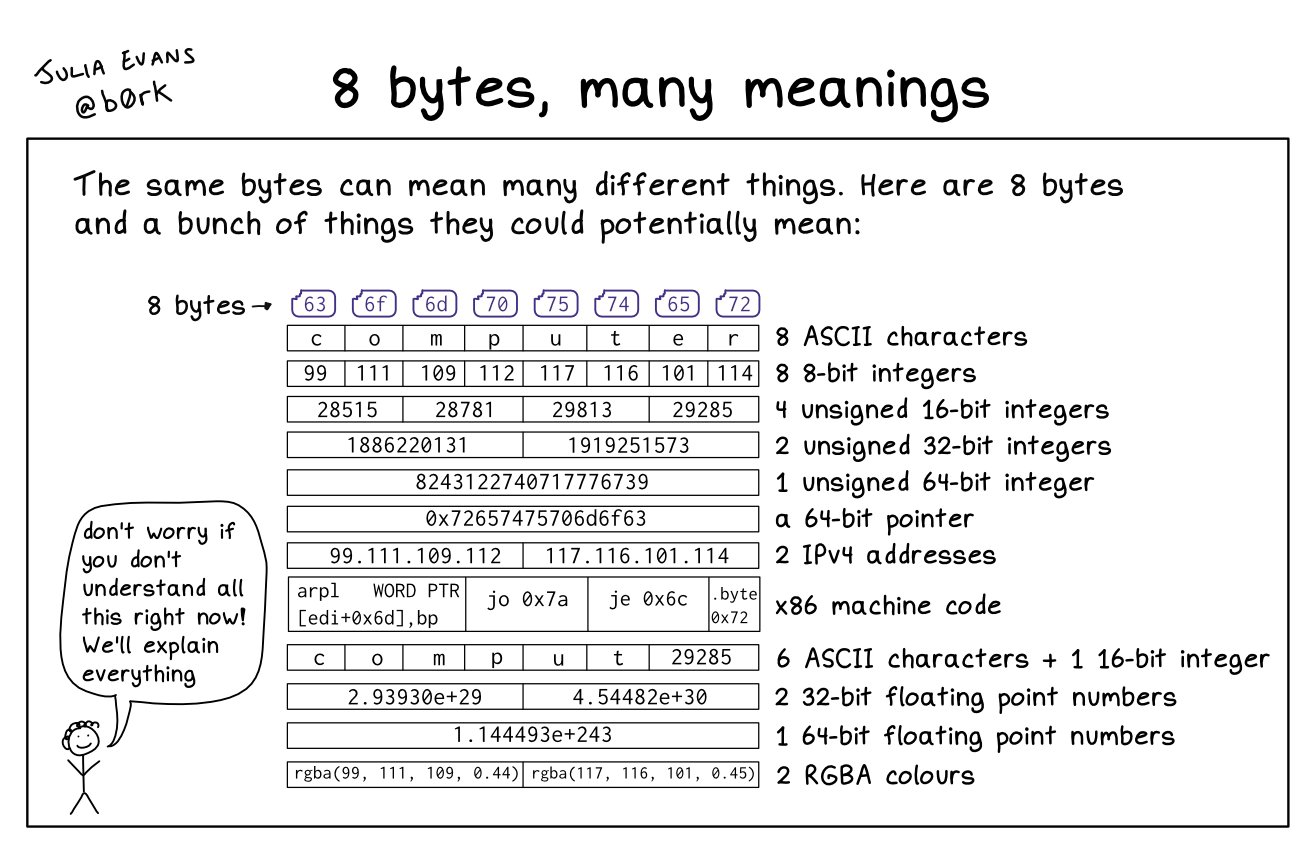
\includegraphics[scale=0.256]{DataTypesMeme.jpeg}
\footnotesize Source: \url{https://twitter.com/b0rk/status/1623041736242040872/photo/1}
\attachfile[zoom=false]{DataTypesMeme.jpeg}
\end{frame}

\end{document}